%========================================================================================
% TU Dortmund, Informatik Lehrstuhl VII
%========================================================================================
\chapter{Spiel}
\label{Spiel}
%
In diesem Abschnitt wird das Snake Spiel beschrieben und die Funktionen von Elementen im Gameplay oder Buttons erklärt. Dabei wird gar nicht auf die Implementierung eingegangen, sondern nur erklärt wie das Spiel funktioniert.


\section{Spiel - Hauptmenü}
\label{Spiel_-_Hauptmenü}
%
\begin{figure}[h]
 \centering
 \includegraphics[scale=0.5]{bilder/Hauptmenü}
 \caption{Hauptmenü}
 \label{fig:hauptmenü}
\end{figure}
Das Hauptmenü \ref{fig:hauptmenü} erscheint beim starten des Spiels und hat fünf Buttons. Liegt der Mauszeiger über dem Fragezeichen-Button wird eine Anleitung des Spiels angezeigt. Dort wird die Steuerung für die jeweiligen Spieler angezeigt und spezielle Elemente aus dem Mehrspielermodus erklärt.\\
\begin{minipage}[X]{1.1\textwidth}
 \centering
 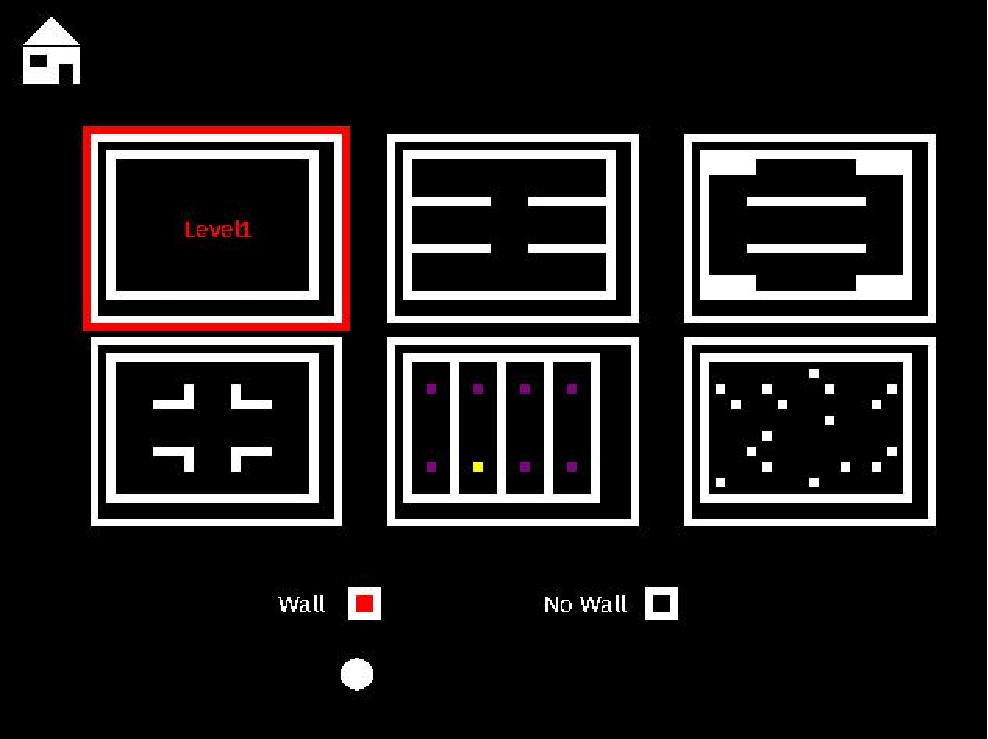
\includegraphics[scale=0.5]{bilder/Einstellungen}
 \captionof{figure}{Einstellungen}
 \label{fig:einstellungen}
\end{minipage}
\newline \\ \\
Wird auf das Zahnrad rechts oben geklickt, öffnet sich das Einstellungsmenü \ref{fig:einstellungen}, indem verschiedene Levels ausgewählt werden können und die Außenwand aktiviert und deaktiviert werden kann. Ist die Außenwand deaktiviert, kann die Schlange beim kollidieren mit der Außenwand nicht sterben. Durch klicken auf das Haus links oben kehrt der Spieler zum Hauptmenü zurück.\newline \newline \\ 
\begin{minipage}[X]{1.1\textwidth}
 \centering
 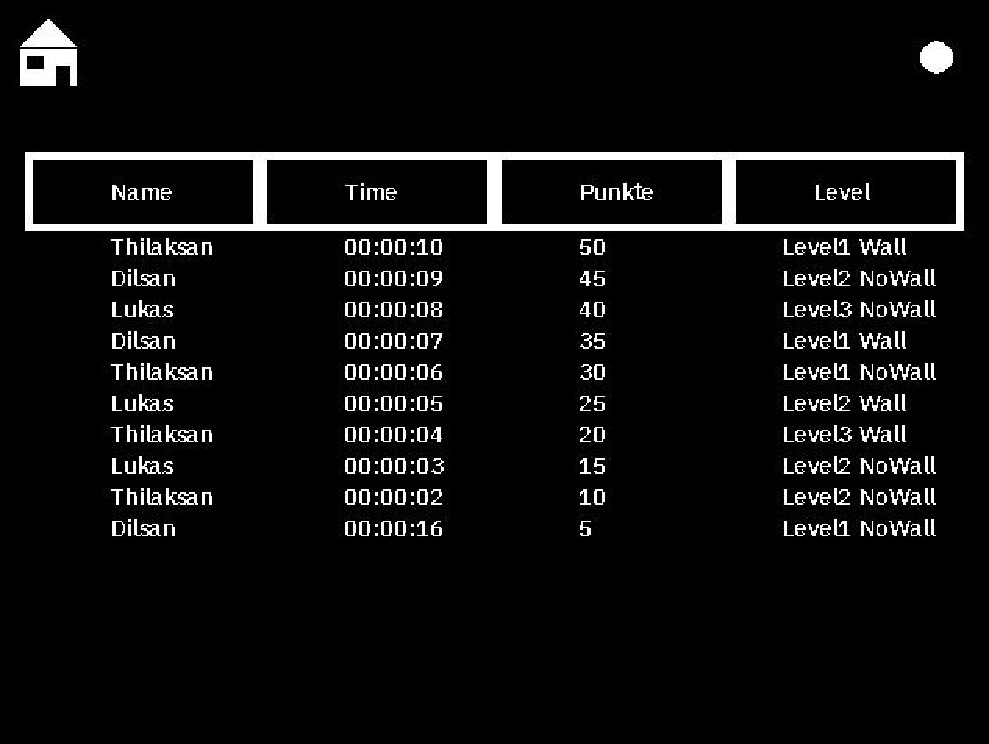
\includegraphics[scale=0.5]{bilder/Highscore}
 \captionof{figure}{Highscore}
 \label{fig:highscore}
\end{minipage}
\newline \\ \\
Wird im Hauptmenü auf den Highscore-Button geklickt, wird der Highscore \ref{fig:highscore} aus den bisher gespielten Spielen angezeigt. Dabei sind die Highscores primär nach Punkten und sekundär nach Zeit sortiert. Außerdem steht in jeweils der letzten Zeile der Highscores das Level, indem gespielt wurde. Mit Klicken auf das Haus links oben kehrt der Spieler zurück zum Hauptmenü.
\\
 Klickt der Spieler auf den "One Player Game"-Button öffnet sich ein Menü, indem der Spieler seinen Namen eintragen kann. Dies kann durch Klicken auf die jeweiligen Buttons auf dem Bildschirm oder durch Eingabe über die Tastatur geschehen. Das Spiel wird dann gestartet, wenn der StartGame-Button betätigt wurde. Wählt der Spieler den Mehrspielermodus, durch Betätigen des "Two Player Game"-Button im Hauptmenü, öffnet sich wieder ein Menü zum Eintragen der Spielernamen und das Spiel kann durch das Betätigen des StartGame-Buttons gestartet werden.  


\section{Spiel - Einzelspielermodus}
\label{Spiel_-_Einzelspielermodus}
%
\begin{figure}[h]
 \centering
 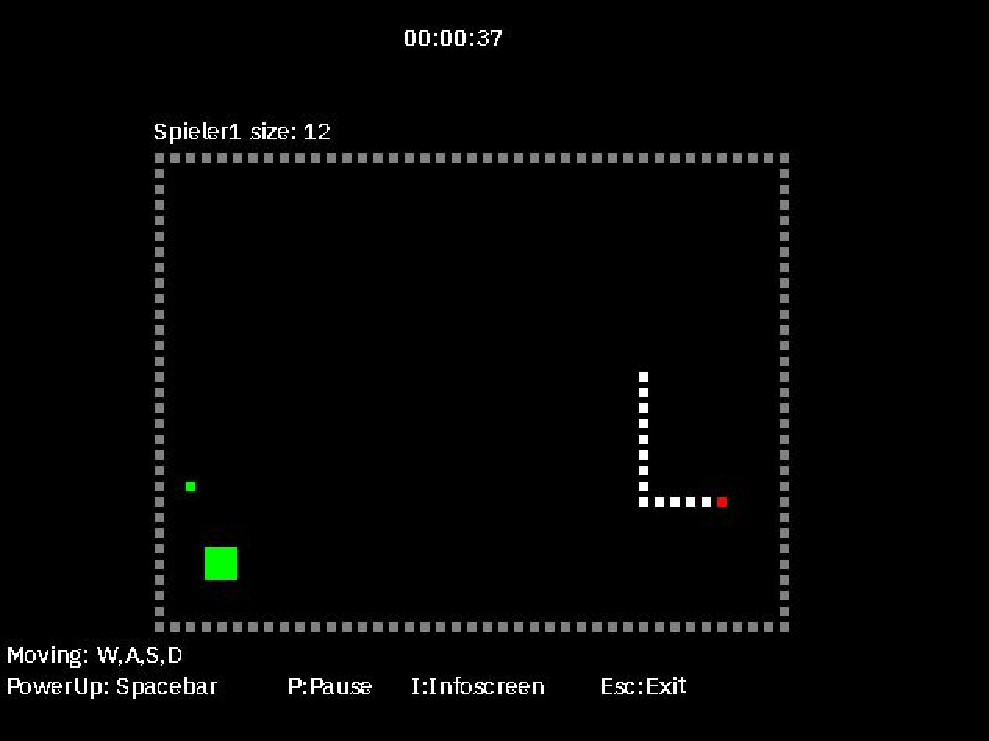
\includegraphics[scale=0.5]{bilder/Einzelspielermodus}
 \caption{Einzelspieler Spiel}
 \label{fig:einzelspielermodus}
\end{figure}
	Der Einzelspielermodus ist im Grunde das traditionelle Snake Game. Die Schlange lässt sich steuern durch Betätigen der Tasten A,S,D,F und bewegt sich alle fünf Frames. Die grünen Elemente sind das Essen der Schlange, welches die Schlange wachsen lässt. Dabei wächst die Schlange um eine Größe beim Verzehren des kleinen Food-Elements und um zwei beim Verzehren des großen Superfood-Elements.
	Das Spiel kann durch die entsprechenden Levels erschwert werden.Level fünf hat ein lilanes Teleport-Element, welches die Schlange zu einem anderen Teleport-Element teleportiert. Dabei teleportieren die oberen Elemente zum nächsten rechten Element und die unteren Elemente zum nächsten linkem Element. Level 6 verändert sein inneres Wandmuster nach dem Verzehren des Food-Elements jedoch nicht nach Verzehren des Superfood-Elements. Das Spiel endet, wenn die Schlange mit der Wand oder mit sich selber kollidiert.   


\section{Spiel - Mehrspielermodus}
\label{Spiel_-_Mehrspielermodus}
%
\textcolor{white}{easily}
\newline 
\begin{minipage}[X]{1.0\textwidth}
 \centering
 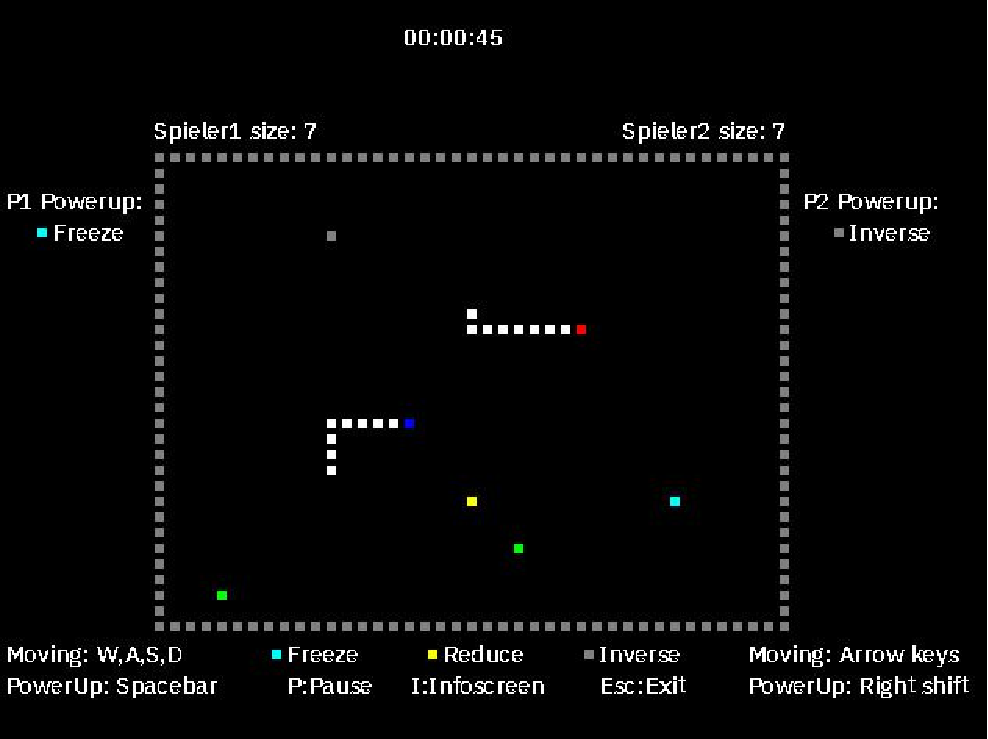
\includegraphics[scale=0.5]{bilder/Mehrspielermodus}
 \captionof{figure}{Mehrspieler Spiel}
 \label{fig:mehrspielermodus}
\end{minipage}
\\ \\ 
	Beim Mehrspielermodus spielen zwei Spieler gegeneinander und versuchen das Spiel durch töten der Schlange des Gegenspielers zu gewinnen. Spieler eins bewegt die rote Schlange mit den Tasten A,S,D,F und Spieler zwei bewegt die blaue Schlange mit den Pfeiltasten. Im Mehrspielermodus gibt es außerdem Spezial-Elemente, wie das cyanfarbene Freeze-Element, das gelbe Reduce-Element und das graue Inverse Element. Diese Elemente können aufgesammelt werden und mit Leertaste für Spieler eins und mit Shift für Spieler zwei eingesetzt werden. Dabei kann nur ein Element gleichzeitig in der Tasche eines jeweiligen Spielers sein. Beim Einsatz des Freeze-Elementes kann die gegnerische Schlange sich für 25 Frames nicht bewegen. Beim Einsatz des Reduce Elementes veringert sich die Länge der gegnerischen Schlange um eine Größe. Das Inverse-Element invertiert die Steuerung des Gegenspielers für 250 Frames. Das Spiel ist beendet, wenn eines der Spieler verliert. Kollidiert die Schlange eines Spielers mit der Wand, sich selber oder dem Körper der gegnerischen Schlange, verliert derjenige Spieler. Kollidieren beide Schlangen Kopf an Kopf gewinnt derjenige Spieler mit der größeren Schlange.  

\section{Spiel - Spielende}
\label{Spiel_-_Spielende}
%
\textcolor{white}{easily}
\newline 
\begin{minipage}[X]{1.1\textwidth}
 \centering
 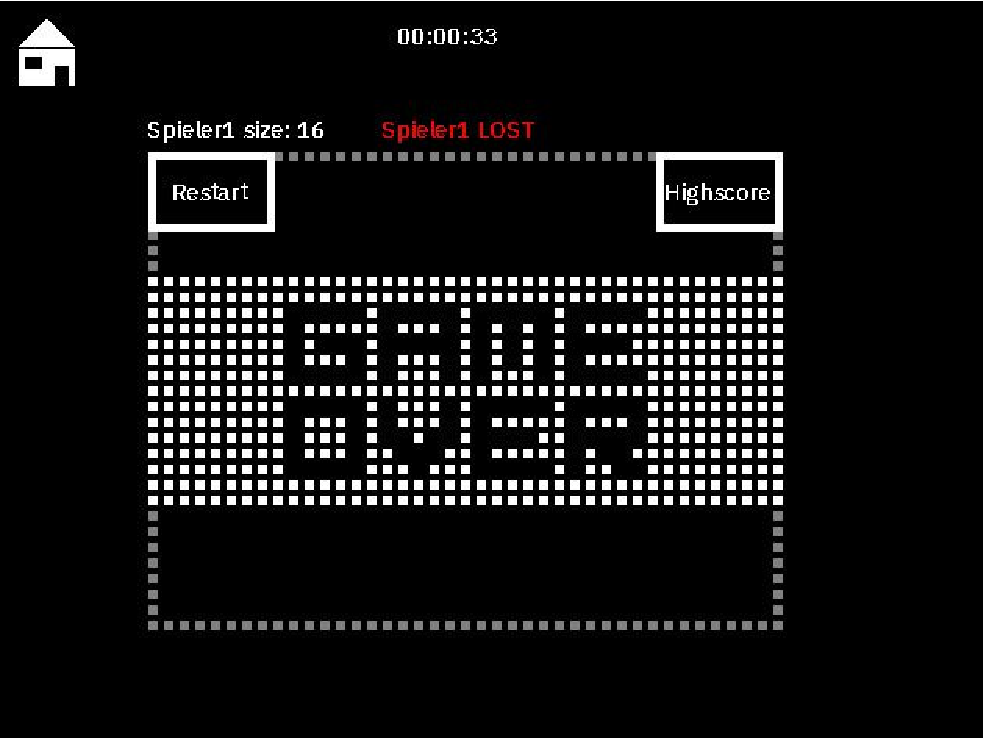
\includegraphics[scale=0.5]{bilder/Spielende}
 \captionof{figure}{Spielende}
 \label{fig:spielende}
\end{minipage}
\\ \\ 
	Ist das Spiel zu Ende erscheint eine kleine Animation und mehrere Buttons. Der Restart-Button startet das Spiel neu und der Highscore-Button zeigt den Highscore an. Außerdem steht über dem Spielfeld welcher Spieler gewonnen hat.  

%
